\subsection{Particle identification}
\begin{figure}[htbp]
  \centering
  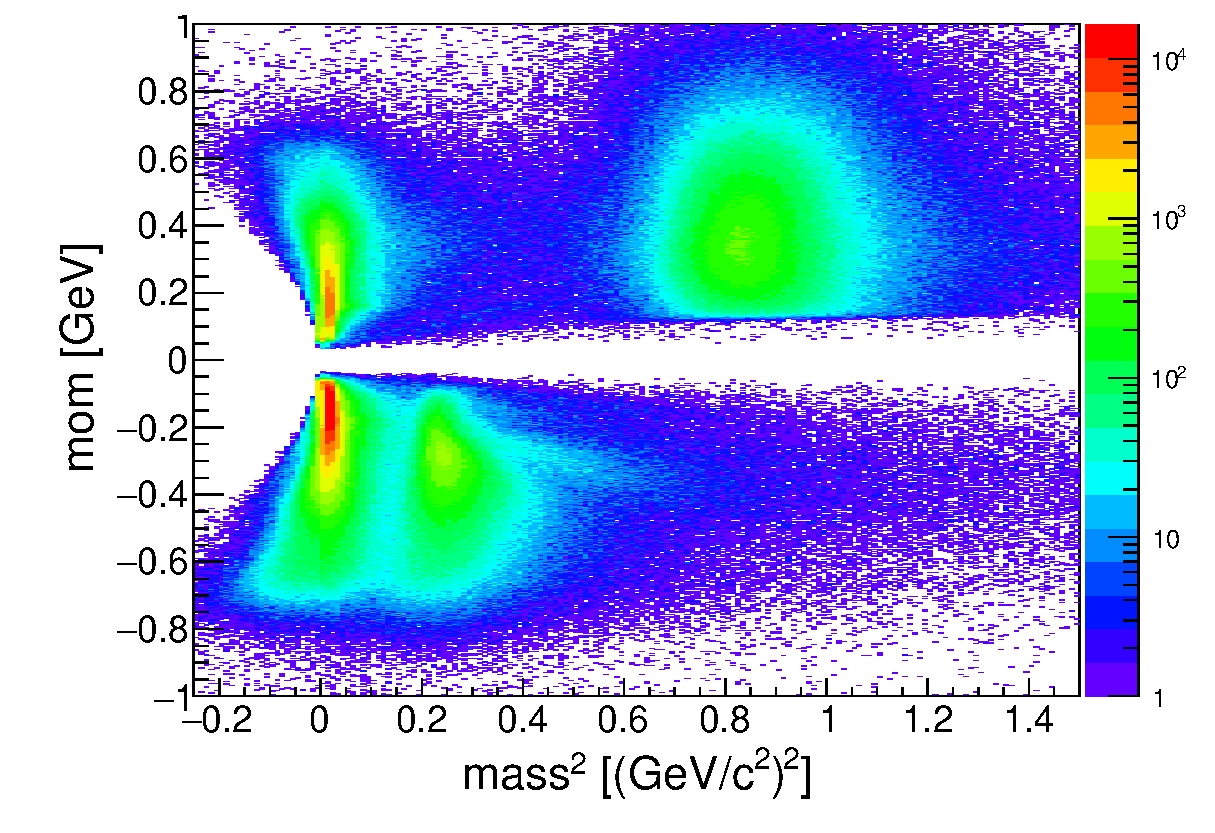
\includegraphics[width=8cm]{../pic/Run78/CDS/pid.eps}
  \caption{
    This figure shows scattered plot of mass square and momentum.
    Mass square was calculated by the Eq.\ref{eq:CDS_mass2}.
    Sign of the momentum means particle charge so, plus means positive charged particle and minus means negative charged particle.
  }
  \label{fig:CDS_PID}
\end{figure}

Decay particle was identified by the velocity calculated from the T0-CDH time-of-flight and the momentum evaluated from the curvature of magnetic field.
The velocity $\beta$ was calculated using below equation
\begin{equation}
  \beta=\frac{1}{c}\frac{L_{Vertex-CDH}}{(TOF_{CDH-T0}-T^{calc}_{T0-Vertex})}
\end{equation}
The $L_{Vertex-CDH}$ is the flight-length from the T0 to the CDH, which was calculated from line distance from the the T0 to the reaction vertex
and helix distance from the vertex to the CDH hit position.
The $T^{calc}_{T0-Vertex}$ mean the calculated time from the T0 to the reaction vertex point using beam momentum analyzed by the D5 magnet with energy loss correction of the materials at beam trajectory.
Decay charged particles were identified by the mass square which calculated by the Eq.\ref{eq:CDS_mass2} and the momentum. 
\begin{equation}
  m^{2}=p^2\times\frac{1-\beta^2}{\beta^2} \label{eq:CDS_mass2}
\end{equation}


